\pdfoutput=1 
\documentclass[10pt,conference]{IEEEtran}

\usepackage[T1]{fontenc} % optional
\usepackage{amsmath,amssymb,amsfonts}
%\usepackage[cmintegrals]{newtxmath}
\usepackage{cite}
\usepackage{algorithmic}
\usepackage{graphicx}
\usepackage{textcomp}
\usepackage{xcolor}
\usepackage{multirow}
\usepackage{subcaption}
\usepackage{lipsum}

%\setcitestyle{nocompress}
\usepackage[normalem]{ulem}
%\usepackage[numbers,sort]{natbib}

\usepackage{todonotes}
\usepackage{url}
\usepackage{graphicx}
\usepackage{xspace}
\usepackage{tikz,pgfplots}

\usepgfplotslibrary{statistics}


\newcommand{\system}{\textsc{Groot}\xspace}


\newcommand{\aftertao}[1]{{\color{blue}#1}}

\begin{document}

\title{Groot: An Event-graph-based Approach for Root Cause Analysis in Industrial Settings}

\author{
\IEEEauthorblockN{Hanzhang Wang\IEEEauthorrefmark{1}, Zhengkai Wu\IEEEauthorrefmark{2},
Huai Jiang\IEEEauthorrefmark{1},
Yichao Huang\IEEEauthorrefmark{1},
\\Jiamu Wang\IEEEauthorrefmark{1},
Selcuk Kopru\IEEEauthorrefmark{1},
Tao Xie\IEEEauthorrefmark{4}}
%\vspace{0.05in}
\IEEEauthorblockA{\IEEEauthorrefmark{1}eBay, \IEEEauthorrefmark{2}University of Illinois at Urbana-Champaign, \IEEEauthorrefmark{4}Peking University}

\IEEEauthorblockA{Email: \{hanzwang,huajiang,yichhuang,jiamuwang,skopru\}@ebay.com,
 zw3@illinois.edu,
%\IEEEauthorrefmark{6}huajiang@ebay.com,
%\IEEEauthorrefmark{7}yichhuang@ebay.com,
%\IEEEauthorrefmark{8}\\jiamuwang@ebay.com,
%\IEEEauthorrefmark{9}skopru@ebay.com,
taoxie@pku.edu.cn}
%\vspace{0.05in}
}

\maketitle

\begingroup\renewcommand\thefootnote{\textsection}
\footnotetext{Tao Xie is also affiliated with Key Laboratory of High Confidence Software Technologies (Peking University), Ministry of Education, China. Hanzhang Wang is the corresponding author.}
%Zhengkai Wu's work is supported in part by NSF grant no. CCF-1816615.}
\endgroup
%\thispagestyle{plain}
%\pagestyle{plain}

\begin{abstract}

For large-scale distributed systems, it is crucial to efficiently diagnose the root causes of incidents to maintain high system availability. The recent development of microservice architecture brings three major challenges (i.e., complexities of operation, system scale, and monitoring) to root cause analysis (RCA) in industrial settings. To tackle these challenges, in this paper, we present \system, an event-graph-based approach for RCA. \system constructs a real-time causality graph based on events that summarize various types of metrics, logs, and activities in the system under analysis. Moreover, to incorporate domain knowledge from site reliability engineering (SRE) engineers, \system can be customized with user-defined events and domain-specific rules. Currently, \system supports RCA among \textit{5,000} real production services and is actively used by the SRE teams in eBay, a global e-commerce system serving more than \textit{159 million} active buyers per year. Over 15 months, we collect a data set containing labeled root causes of 952 real production incidents for evaluation. The evaluation results show that \system is able to achieve 95\% top-3 accuracy and 78\% top-1 accuracy. To share our experience in deploying and adopting RCA in industrial settings, we conduct a survey to show that users of \system find it helpful and easy to use. We also share the lessons learned from deploying and adopting \system to solve RCA problems in production environments.

% Groot firstly construct application run-time application dependency graph; then connects "events" such as developer activities, and distributed low-level monitoring events generated by real-time anomaly detection models; and do root cause analysis at the event level on a dynamic event graph.
\end{abstract}

\begin{IEEEkeywords}
microservices, root cause analysis, AIOps, observability
\end{IEEEkeywords}

% !TEX root = ../arxiv.tex

Unsupervised domain adaptation (UDA) is a variant of semi-supervised learning \cite{blum1998combining}, where the available unlabelled data comes from a different distribution than the annotated dataset \cite{Ben-DavidBCP06}.
A case in point is to exploit synthetic data, where annotation is more accessible compared to the costly labelling of real-world images \cite{RichterVRK16,RosSMVL16}.
Along with some success in addressing UDA for semantic segmentation \cite{TsaiHSS0C18,VuJBCP19,0001S20,ZouYKW18}, the developed methods are growing increasingly sophisticated and often combine style transfer networks, adversarial training or network ensembles \cite{KimB20a,LiYV19,TsaiSSC19,Yang_2020_ECCV}.
This increase in model complexity impedes reproducibility, potentially slowing further progress.

In this work, we propose a UDA framework reaching state-of-the-art segmentation accuracy (measured by the Intersection-over-Union, IoU) without incurring substantial training efforts.
Toward this goal, we adopt a simple semi-supervised approach, \emph{self-training} \cite{ChenWB11,lee2013pseudo,ZouYKW18}, used in recent works only in conjunction with adversarial training or network ensembles \cite{ChoiKK19,KimB20a,Mei_2020_ECCV,Wang_2020_ECCV,0001S20,Zheng_2020_IJCV,ZhengY20}.
By contrast, we use self-training \emph{standalone}.
Compared to previous self-training methods \cite{ChenLCCCZAS20,Li_2020_ECCV,subhani2020learning,ZouYKW18,ZouYLKW19}, our approach also sidesteps the inconvenience of multiple training rounds, as they often require expert intervention between consecutive rounds.
We train our model using co-evolving pseudo labels end-to-end without such need.

\begin{figure}[t]%
    \centering
    \def\svgwidth{\linewidth}
    \input{figures/preview/bars.pdf_tex}
    \caption{\textbf{Results preview.} Unlike much recent work that combines multiple training paradigms, such as adversarial training and style transfer, our approach retains the modest single-round training complexity of self-training, yet improves the state of the art for adapting semantic segmentation by a significant margin.}
    \label{fig:preview}
\end{figure}

Our method leverages the ubiquitous \emph{data augmentation} techniques from fully supervised learning \cite{deeplabv3plus2018,ZhaoSQWJ17}: photometric jitter, flipping and multi-scale cropping.
We enforce \emph{consistency} of the semantic maps produced by the model across these image perturbations.
The following assumption formalises the key premise:

\myparagraph{Assumption 1.}
Let $f: \mathcal{I} \rightarrow \mathcal{M}$ represent a pixelwise mapping from images $\mathcal{I}$ to semantic output $\mathcal{M}$.
Denote $\rho_{\bm{\epsilon}}: \mathcal{I} \rightarrow \mathcal{I}$ a photometric image transform and, similarly, $\tau_{\bm{\epsilon}'}: \mathcal{I} \rightarrow \mathcal{I}$ a spatial similarity transformation, where $\bm{\epsilon},\bm{\epsilon}'\sim p(\cdot)$ are control variables following some pre-defined density (\eg, $p \equiv \mathcal{N}(0, 1)$).
Then, for any image $I \in \mathcal{I}$, $f$ is \emph{invariant} under $\rho_{\bm{\epsilon}}$ and \emph{equivariant} under $\tau_{\bm{\epsilon}'}$, \ie~$f(\rho_{\bm{\epsilon}}(I)) = f(I)$ and $f(\tau_{\bm{\epsilon}'}(I)) = \tau_{\bm{\epsilon}'}(f(I))$.

\smallskip
\noindent Next, we introduce a training framework using a \emph{momentum network} -- a slowly advancing copy of the original model.
The momentum network provides stable, yet recent targets for model updates, as opposed to the fixed supervision in model distillation \cite{Chen0G18,Zheng_2020_IJCV,ZhengY20}.
We also re-visit the problem of long-tail recognition in the context of generating pseudo labels for self-supervision.
In particular, we maintain an \emph{exponentially moving class prior} used to discount the confidence thresholds for those classes with few samples and increase their relative contribution to the training loss.
Our framework is simple to train, adds moderate computational overhead compared to a fully supervised setup, yet sets a new state of the art on established benchmarks (\cf \cref{fig:preview}).

\section{Related Work}\label{sec:related}
 
The authors in \cite{humphreys2007noncontact} showed that it is possible to extract the PPG signal from the video using a complementary metal-oxide semiconductor camera by illuminating a region of tissue using through external light-emitting diodes at dual-wavelength (760nm and 880nm).  Further, the authors of  \cite{verkruysse2008remote} demonstrated that the PPG signal can be estimated by just using ambient light as a source of illumination along with a simple digital camera.  Further in \cite{poh2011advancements}, the PPG waveform was estimated from the videos recorded using a low-cost webcam. The red, green, and blue channels of the images were decomposed into independent sources using independent component analysis. One of the independent sources was selected to estimate PPG and further calculate HR, and HRV. All these works showed the possibility of extracting PPG signals from the videos and proved the similarity of this signal with the one obtained using a contact device. Further, the authors in \cite{10.1109/CVPR.2013.440} showed that heart rate can be extracted from features from the head as well by capturing the subtle head movements that happen due to blood flow.

%
The authors of \cite{kumar2015distanceppg} proposed a methodology that overcomes a challenge in extracting PPG for people with darker skin tones. The challenge due to slight movement and low lighting conditions during recording a video was also addressed. They implemented the method where PPG signal is extracted from different regions of the face and signal from each region is combined using their weighted average making weights different for different people depending on their skin color. 
%

There are other attempts where authors of \cite{6523142,6909939, 7410772, 7412627} have introduced different methodologies to make algorithms for estimating pulse rate robust to illumination variation and motion of the subjects. The paper \cite{6523142} introduces a chrominance-based method to reduce the effect of motion in estimating pulse rate. The authors of \cite{6909939} used a technique in which face tracking and normalized least square adaptive filtering is used to counter the effects of variations due to illumination and subject movement. 
The paper \cite{7410772} resolves the issue of subject movement by choosing the rectangular ROI's on the face relative to the facial landmarks and facial landmarks are tracked in the video using pose-free facial landmark fitting tracker discussed in \cite{yu2016face} followed by the removal of noise due to illumination to extract noise-free PPG signal for estimating pulse rate. 

Recently, the use of machine learning in the prediction of health parameters have gained attention. The paper \cite{osman2015supervised} used a supervised learning methodology to predict the pulse rate from the videos taken from any off-the-shelf camera. Their model showed the possibility of using machine learning methods to estimate the pulse rate. However, our method outperforms their results when the root mean squared error of the predicted pulse rate is compared. The authors in \cite{hsu2017deep} proposed a deep learning methodology to predict the pulse rate from the facial videos. The researchers trained a convolutional neural network (CNN) on the images generated using Short-Time Fourier Transform (STFT) applied on the R, G, \& B channels from the facial region of interests.
The authors of \cite{osman2015supervised, hsu2017deep} only predicted pulse rate, and we extended our work in predicting variance in the pulse rate measurements as well.

All the related work discussed above utilizes filtering and digital signal processing to extract PPG signals from the video which is further used to estimate the PR and PRV.  %
The method proposed in \cite{kumar2015distanceppg} is person dependent since the weights will be different for people with different skin tone. In contrast, we propose a deep learning model to predict the PR which is independent of the person who is being trained. Thus, the model would work even if there is no prior training model built for that individual and hence, making our model robust. 

%


\section{An example}
\label{sec:6}
\begin{figure}[H]

\includegraphics[scale=.6]{schematic}
\centering
\caption{ A sketch of the example constructed in this section. The manifold decomposes into three pieces, left and right caps and a middle region. The loop drawn on the boundary of the left cap only bounds surfaces of high topological complexity that are at least partly contained in the right cap. This ensures the isoperimetric ratio of that loop is very small.}
\label{fig:example_sketch}
\end{figure}

The aim of this section is to show that the first positive eigenvalue of the 1-form Laplacian can vanish exponentially fast in relation to volume. This contrasts the behaviour of the first positive eigenvalue of the Laplacian on functions.

Our construction is similar to that in \cite{BD}. Essentially, we choose a hyperbolic 3-manifold with totally geodesic boundary and glue it to itself using a particular psuedoAnosov with several useful properties. By \cite{BMNS}, this family has geometry that up to bounded error can be understood in terms of a simple model family. Using this model family, we show that one can find curves with uniformly bounded length whose stable commutator length grows exponentially in the volume. We then use the spectral gap upper bound in Theorem A to conclude the first positive eigenvalue vanishes exponentially fast.

Throughout this section, we need to compare geodesic lengths in different submanifolds of a given manifold $M$. Let $|\cdot|_{X}$ denote the geodesic length of a homotopy class of curves relative endpoints in a manifold $X$ and $\text{length}(\cdot)$ be the length in $M$ of the curve. Similarly, when we compute stable commutator length for the fundamental group of a manifold $X$, which may or may not be a submanifold of $M$, we denote it $\scl_X$.

We will need that for certain curves, $\scl$ is comparable to length. We begin with a simple but essential technical lemma.
\begin{figure}[H]
\labellist
\small\hair 2pt
 \pinlabel {$a_0$} [ ] at 830 1100
 \pinlabel {$a_1$} [ ] at 1300 1100
 \pinlabel {$b_0$} [ ] at 830 1250
 \pinlabel {$b_1$} [ ] at 1300 1250
 \pinlabel {$t_1$} [ ] at 380 1290
 \pinlabel {$t_0$} [ ] at 380 1120
\endlabellist
\centering
\includegraphics[width = 15cm]{lemdiagram}
\caption{ Illustrating Lemma \ref{lem:6.1} , the rectangular base of the figure is part of the totally geodesic surface $S$ and the box is the corresponding part of the tubular neighborhood $N_\e(S)$ foliated by surfaces $S_t$ parallel to $S$. Drawn in the box is the surface $\Sigma$, which is transverse the foliation except at isolated points. The multicurve $a_0\cup a_1$ is part of a single level set $S_{t_0} \cap \Sigma$, but only $a_0$ is part of the curve $c_{t_0}$ described in the lemma, whereas the multicurve $b_0\cup b_1$ forms the multicurve $c_{t_1}$ in the lemma.}
\label{fig:box}
\end{figure}


\begin{lem} \label{lem:6.1} Let $M$ be a compact hyperbolic 3-manifold with totally geodesic boundary $ \d M = S$. Let $\e$ be smaller than the injectivity radius of $M$ and such that $N_\e(S)$ is an embedded tubular neighborhood. Let $\{S_t\}$ be the leaves of the foliation of $N_\e(S)$ by surfaces equidistant from $S$.  Let $\Sigma$ be a smooth incompressible proper not necessarily immersed surface in $M$ that is transverse to the foliation $\{S_t\}$ except at isolated points. Let $c = \d \Sigma$. By transversality, for generic $t$ the multicurve $c_t$ given by the part of $S_t\cap \Sigma$ that cobounds a subsurface of $\Sigma$ with $c = c_0$ is a smooth multicurve.  Let $T$ be the set (of full measure) of all $t\in[0,\e)$ such that $c_t$ is a smooth multicurve. Since $S$ is totally geodesic, each multicurve $c_t$ is homotopic to a possibly degenerate geodesic multicurve $\gamma_t$ in $S$. Let $\Sigma_\e$ be the part of $\Sigma$ contained in $N_\e(S)$. Then for $C = 1/\e$, we have that $$\inf\limits_{t\in T} |\gamma_t|_{S} \leq C \emph{Area}(\Sigma_\e).$$
\end{lem}

\begin{proof} The coarea formula implies the inequality $\inf\limits_{t\in T} |c_t|_{S_t} \leq C \text{Area}(\Sigma_\e)$.  Since $S$ is totally geodesic, for all $t\in T$, we have $|\gamma_t|_S\leq |c_t|_{S_t}.$  \end{proof}
Note that in the previous lemma, when $\inf\limits_{t\in T} |\gamma_t|_S$ is zero, because $\Sigma$ is incompressible and any loop with length less than $\inj(M)$ bounds a disk, every component of $\Sigma$ can either be homotoped to be disjoint from $N_\e(S)$ or be contained in $S$.

The next proposition requires a notion of geometric complexity for homology classes. For any compact Riemannian manifold $M$ one can define the stable norm on the first homology of $M$ (see \cite{Gromovmetric} Section 4C). The mass of a Lipschitz 1-chain $\alpha = \sum_i t_i\alpha_i$ in $M$ is defined to be $\text{mass}(\alpha) = \sum_i |t_i|\text{length}(\alpha_i).$ The mass of a class $a\in H_1(M)$ is then the infimal value of the mass of a chain $\alpha$ representing $a$.
For a class $a\in H_1(M)$, the stable norm of $a$ is then given by $$||a||_{s,M} = \inf\limits_{m>0}\frac{\text{mass}(m a)}{m}.$$

Stable commutator length can also be generalized to geodesic multicurves (see Section 2.6 of \cite{Calegari}), which can naturally be viewed as Lipschitz chains. Suppose $\gamma_i\in \pi_1 M$ and $ \sum_i n [\gamma_i] = 0$ in $H_1(M)$. Let $\gamma$ be the geodesic multicurve, which is not necessarily simple, consisting of the geodesic loops determined by $\gamma_i$. Say a surface $f:S\to M$ is admissible of degree $n(S)$ if it has no closed components and $\d S$ is a union of circles $S^1_i$ with $f|_{S^1_i}$ a degree $n(S)$ cover of $\gamma_i$.
Then we define stable commutator length of $\gamma$ to be $$\scl(\gamma) = \inf\limits_{S \text{ admissible}} \frac{\chi_-(S)}{2n(S)}.$$ When $\gamma$ is a single loop, this definition agrees with the usual definition of stable commutator length.

 \begin{prop} \label{prop:6.2} Let $M$ be a compact oriented hyperbolic 3-manifold with totally geodesic boundary $\d M = S$. Let $\gamma$ be a geodesic multicurve in $S$ that is rationally nullhomologous in $M$. Then there is a constant $D> 0$ depending only on $M$ such that $$||[\gamma]||_{s,S}\leq D\scl_M(\gamma).$$ \end{prop}

 \begin{proof} If $\gamma$ is nullhomologous in $S$, then the left hand side is zero and the inequality holds. Assume now that $[\gamma]\neq 0\in H_1(S)$. Fix $\delta>0$. Let $\Sigma_m$ be an incompressible admissible surface for $\gamma$ of degree $m = n(S)$ such that $\chi_-(\Sigma_m)/2m -\scl(\gamma) < \delta$. We can triangulate $\Sigma_m$ so that there is a single vertex on each boundary component. This triangulation has $4g +3b - 4$ faces, where $g$ is the genus of $\Sigma_m$ and $b$ the number of boundary components. We can then straighten this triangulation to obtain a piecewise totally geodesic triangulated surface. Replace $\Sigma_m$ with this surface. Since every face of this triangulation of $\Sigma_m$ is geodesic, every face has area at most $\pi$. Since there are $4g+3b - 4$ faces and $\chi_-(\Sigma_m) = 2g-2 + b$, we can estimate  $$\text{Area}(\Sigma_m) \leq 3\pi\chi_-(\Sigma_m).$$

We can perturb $\Sigma_m$ to obtain a smooth surface $\Sigma’_m$ that it is transverse the foliation of $N_\e(S)$ except at isolated points and in doing so increase the area by less than $\delta$. Let $\gamma_t$ be the family of multicurves in Lemma \ref{lem:6.1}  applied to $\Sigma’_m$. Since each curve $\gamma_t$ cobounds a surface in $S$ with $\d \Sigma_m$, they are homologous, thus $||[\gamma_t]||_{s,S} = m||[\gamma]||_{s,S}$. Since $||[\gamma_t]||_{s,S}\leq |\gamma_t|_S$,
Lemma \ref{lem:6.1}  implies that $$m||[\gamma]||_{s,S}\leq C\text{Area}(\Sigma_m’) \leq C \text{Area}(\Sigma_m) + C\delta \leq 3C\pi\chi_-(\Sigma_m) + C\delta.$$
From this we get  $$||[\gamma]||_{s,S}\leq 6C\pi\chi_-(\Sigma_m)/2m + C\delta/m\leq 6C\pi\scl_M(\gamma) + 6C\pi\delta +C\delta/m.$$
Since the stable commutator length of a nontrivial rational commutator is bounded away from zero by a constant only depending on $M$, by Theorem 3.9 in \cite{Calegari}, we can replace $C$ with a larger constant $D$ such that $$||[\gamma]||_{s,S}\leq D\scl_M(\gamma),$$ as desired. \end{proof}

 We now introduce the family of manifolds that we use in our construction. The family $\{W_n\}$ of manifolds we study are easily understood using the model manifold theory of \cite{BMNS}. In particular, there is a $K$-biLipschitz map between $W_n$ and a model manifold $M_n$, where $K$ is independent of $n$. The base of the construction is Thurston’s tripus manifold $W$ (see \cite{thurstonbook}, Section 3.3.12), a hyperbolic manifold with totally geodesic boundary, and a psuedoAnosov homeomorphism $f$ of the boundary surface $\d W$. The model manifold $ M_n$ is a degree $n$ cyclic cover of the mapping torus $M_{f}$ cut open along a fiber with two oppositely oriented copies of $W$, denoted $W^+$ and $W^-$ glued as described in \cite{BMNS} Section 2.15 to the two boundary components of the cut open mapping torus. This decomposes $W_n$ into three pieces, a product region $S\times [0, n]$ and the caps $W^+$ and $W^-$ in a metrically controlled way. It will be convenient to set $M^+ = W^+\subset M_n$ and $M^- = W^-\subset M_n$ when talking about the caps of the model manifold $M_n$ for fixed $n$, and to let $W^+$ and $W^-$ denote the images of these spaces under the natural inclusion into $W_n$.

 \vspace{1cm}
\begin{figure}[H]
\labellist
\small\hair 2pt
 \pinlabel {$M^+$} [ ] at 950 1100
 \pinlabel {$M^-$} [ ] at 2000 1100
 \pinlabel {$S\times[0,n]$} [ ] at 1500 1600
\endlabellist
\centering
\includegraphics[scale=.15]{modelscheme}
\caption{ A schematic picture of the model manifold $M_n$ with caps $M^+$ and $M^-$ two oppositely oriented copies of the tripus manifold.}
\label{fig:caps_schematic}
\end{figure}

Given a multicurve $c$ in $M^{\pm}$, we say $c$ \textbf{bounds on both sides} if there are incompressible surfaces $S^+$ in $M^+$ and $S^-$ in $M^-$ both with boundary homotopic to $c$.

We encode the construction and its essential properties in the following proposition.

\begin{prop}  \label{prop:6.3}There is a family $\{W_n\}$ of closed hyperbolic 3-manifolds with injectivity radius uniformly bounded below and volume growing linearly in $n$ constructed from the tripus and a pseudoAnosov $f$ as described above. Each manifold $W_n$ is $K$-biLipschitz equivalent to the model manifold $M_n$ for some constant $K$ independent of $n$. Any homologically nontrivial loop in $H_1(\d W^{\pm})$ that bounds a surface in $M^{\pm}$ cannot bound on both sides. The pseudoAnosov $f$ is such that for any nonzero class $a\in H_1(\d W^+)$, the stable norm of $f_*^n(a)$ grows exponentially.
\end{prop}

\begin{proof}
Let $W$ be Thurston’s tripus manifold, a compact hyperbolic 3-manifold with totally geodesic boundary a genus 2 surface for which the inclusion map $H_1(\d W;\Z)\to H_1(W;\Z)$ is onto.
The homology of the boundary $\d W$ decomposes as the direct sum of rank 2 submodules $U$ and $V$, where $V\subset H_1(\d W)$ is the image of the boundary map $\d : H_2(W,\d W;\Z)\to H_1(\d W;\Z)$ (which is also the kernel of the inclusion $H_1(\d W)\to H_1(W)$) and $U$ is a compliment of $V$ (note that the inclusion map $H_1(\d W)\to H_1(W)$ restricted to $U$ is an isomorphism).
Let $S$ be a genus 2 surface, which we will use to mark the boundaries of $W^{+}$ and $W^-$. Assume $H_1(S;\Z)$ is generated by $e_1,~e_2,~e_3,~e_4$. Choose a marking $S\to \d W^+$ so in $W^+$ one has $U = \langle e_1,e_2\rangle $ and $V = \langle e_3, e_4\rangle$.
Similarly, choose a marking $S\to \d W^-$ so that in $W^-$ one has $V = \langle e_1,e_2\rangle $ and $U = \langle e_3, e_4\rangle$. We then define $$W_n = W^+\cup_{f^n}W^-$$ where $f:S\to S$ is a pseudo-Anosov that acts on $H_1(S)$ by the symplectic matrix\[ F = \begin{pmatrix}
 2 &  1 & 0 & 0 \\
 1 & 1 & 0 & 0 \\
 0 & 0 & 1 & -1\\
 0 & 0 & -1 & 2
\end{pmatrix} \] For the existence of such a pseudoAnosov mapping class, see the proof Lemma 7.1 in \cite{BD}. This matrix preserves the subspace decomposition above, and so ensures that every curve in $\d W^{\pm}$ that is not nullhomologous in $\d W^{\pm}$ but bounds a surface in $M^{\pm}$ cannot bound on both sides.

The mapping class $f$ acts as an Anosov matrix on $U$ and $V$. This ensures the standard Euclidean $\ell^2$-norm $||F^n(a)||_E$ of an element $a\in H_1(S)$ grows exponentially in $n$ (indeed, for our choice of $F$, it grows like $(\frac{3+\sqrt{5}}{2})^n$). Since norms on finite dimensional real vector spaces are comparable, there is a constant comparing the stable norm induced by the metric inherited from $W$ to the standard Euclidean $\ell^2$-norm on $H_1(S)$.

Lemma 7.3 in \cite{BD} explains how Theorem 8.1 in \cite{BMNS} implies that for large $n$ the manifolds $W_n$ admit a $K$-biLipschitz diffeomorphism $\mu$ from the model manifold $ M_n$ as described above. After increasing $K$, we can drop the large $n$ condition. This then also implies the linear volume growth and injectivity radius bounds.
\end{proof}

\begin{remark}
Using the model manifold, one can easily estimate the Cheeger constant of $W_n$, which will decay like $1/n$.
\end{remark}


\begin{mainthm}  \label{thm:C} The family $W_n$ of closed hyperbolic 3-manifolds from Proposition \ref{prop:6.3}  has 1-form Laplacian spectral gap that vanishes exponentially fast in relation to volume:
$$\sqrt{\lambda(W_n)}\leq B\vol(W_n)e^{-r\vol(W_n)},$$
where $r$ and $B$ are positive positive constants and $\lambda(W_n)$ is the first positive eigenvalue of the 1-form Laplacian on $W_n$.
\end{mainthm}


\begin{proof}
We continue using notation introduced in the previous propositions. Take $\gamma$ in $\d M^+\subset M_n$ to be an embedded geodesic loop representing the class $e_1 \in U \subset H_1(\d W^+)$. Recall from the proof of Proposition \ref{prop:6.3} that $\gamma\subset \d M^+$ does not bound a surface in $M^+$ but that $f^n(\gamma)\subset \d M^-$ bounds a surface in $M^-$. Let $\alpha_n = f^n(\gamma)\subset \d M^- \subset M_n$. Note that $\alpha_n$ and $\gamma$ are isotopic in $M_n$.

Fix $\delta>0$. Consider some positive integer $m$ and  incompressible surface $\Sigma_m$ bounding $\alpha_n^m$ in $M_n$ with $\chi_-(\Sigma_m)/2m - \scl_{M_n}(\gamma) < \delta$ and which minimizes $\chi_-$ among surfaces with boundary $\alpha_n^m$. We can then replace $\Sigma_m$ with a homotopic surface that pushes the boundary of $\Sigma_m$ into the interior of $M^-$ and which intersects $\d M^-$ transversely and essentially in both $\d M^-$ and $\Sigma_m$.
We can then attach an annulus to $\Sigma_m$ cobounding $\alpha_n^m$ and the boundary of the modified surface $\Sigma_m$. This new $\Sigma_m$ bounds $\alpha_n^m$ with a collar neighborhood of the boundary contained entirely in $M^-$ and intersects $\d M^-$ transversely in a union of loops essential in both $\Sigma_m$ and $\d M^-$.

We focus on the portion of $\Sigma_m$ that lies in $M^-$. Define $\Sigma^-_m =\Sigma_m\cap M^-$. If $\Sigma_m$ is contained in $M^-$, then Proposition \ref{prop:6.2}  applied to $\alpha_n^m$ in $M^-$ implies that
$$||[\alpha_n^m]||_{s,\d M^-} = m||[\alpha_n]||_{s,\d M^-} \leq m\scl_{M^-}(\alpha_n)\leq D\chi_-(\Sigma_m^-) = D\chi_-(\Sigma_m) ,$$
where $||\cdot||_{s, \d M^-}$ is the stable norm of $H_1(\d M^-)$. Since $\chi_-(\Sigma_m)/m- \scl_{M_n}(\gamma)\leq \delta$, we conclude $$||[\alpha_n]||_{s,\d M^-}\leq D\scl_{M_n}(\gamma) + D\delta.$$

Our goal now is to get this same estimate for the other possible ways $\Sigma_m$ sits in $M_n$.
\vspace{1cm}
\begin{figure}[H]
\labellist
\small\hair 2pt
 \pinlabel {$M^+$} [ ] at 900 1560
 \pinlabel {$S\times[0,n]$} [ ] at 1480 1650
 \pinlabel {$M^-$} [ ] at 2000 1560
 \pinlabel {$\alpha$} [ ] at 1750 1050
\endlabellist
\centering
\includegraphics[scale=.2]{schematic5}
\caption{ A schematic picture of the simplest case of a surface bounding $\alpha$ in $M^-$.}
\label{fig:alpha_bounds}
\end{figure}

Consider the case that $\Sigma_m$ does not lie entirely in $M^-$. There are two possibilities. The first involves the surface $\Sigma_m$ passing into the product region but not intersecting $M^+$. In this case the surface can be homotoped to lie in $M^-$, so that Proposition \ref{prop:6.2} applies, giving the desired estimate as in the previous case.
\vspace{2cm}
\begin{figure}[H]
\labellist
\small\hair 2pt
 \pinlabel {$M^+$} [ ] at 900 1560
 \pinlabel {$S\times[0,n]$} [ ] at 1480 1650
 \pinlabel {$M^-$} [ ] at 2000 1560
 \pinlabel {$\alpha$} [ ] at 1750 850
\endlabellist
\centering

\includegraphics[scale=.2]{schematic3}
\caption{ A schematic picture of a surface bounding $\alpha$ that passes back into $M^-$ but does not pass into $M^+$.}
\label{fig:pass_back_schematic}
\end{figure}

\vspace{2cm}
\begin{figure}[H]
\labellist
\small\hair 2pt
 \pinlabel {$M^+$} [ ] at 900 1560
 \pinlabel {$S\times[0,n]$} [ ] at 1480 1650
 \pinlabel {$M^-$} [ ] at 2000 1560
 \pinlabel {$\alpha$} [ ] at 1750 850
 \pinlabel {$c_1$} [ ] at 1750 1285
 \pinlabel {$c_0$} [ ] at 1750 1070

\endlabellist
\centering

\includegraphics[scale=.2]{schematic6}
\caption{ A schematic picture of a surface bounding $\alpha$ that passes back into $M^+$. Notice the multicurve $c^- = c_0\cup c_1$ bounds surfaces in $M^+$ and $M^-$, so is homologically trivial. }
\label{fig:bounds_both_sides}
\end{figure}



The second possibility concerns the surface $\Sigma_m$ crossing through the product region into $M^+$ with an essential intersection with $\d \Sigma^+$. In this case, we will see that the surface $\Sigma_m^-$ has boundary homologous to $\alpha_n^m$, which will allow us to apply Proposition \ref{prop:6.2} to obtain the desired estimate. By construction, a sufficiently small collar $C$ of the boundary $\d \Sigma_m$ in $\Sigma_m$ maps into $M^-$, so in particular, a subsurface of $\Sigma_m^-$ has some boundary component that maps to $\alpha_n^m$. That boundary component can be closed by attaching a surface $S^-$ that bounds $\alpha_n^m$ in $M^-$ to $\Sigma_m$.
From this, we see that the multicurve $c^- = \d \Sigma^-_m -\alpha_n $ bounds surfaces in $M^+$ and $M^-$.
Thus by Proposition \ref{prop:6.3}, $c^-$ must be homologically trivial in $\d M^{-}$. Let $x = \d\Sigma_m^- = c^- + \alpha_n^m$. Since $c^-$ is nullhomologous, $||[x]||_{s,\d M^-} = ||[\alpha_n^m]||_{s,\d M^-} = m||[\alpha_n]||_{s,\d M^-}.$
By Proposition \ref{prop:6.2} , $||[x]||_{s,\d M^-}\leq D\scl_{M^-}(x).$ Since $x$ is essential in $\Sigma_m$, we get that $\chi_-(\Sigma_m^-) \leq \chi_-(\Sigma_m)$, then using that $\chi_-(\Sigma_m)/2m - \delta \leq \scl_{M_n}(\alpha_n)$,
we obtain $\scl_{M^-}(x) \leq \chi_-(\Sigma_m^-)/2 \leq m\scl_{M_n}(\alpha_n) + \delta m$.
Putting this all together and dividing by $m$, we get that $$||[\alpha_n]||_{s,\d M^-}\leq D\scl_{M_n}(\alpha_n) + D\delta.$$

We therefore have in each case that there is a constant $D$ independent of $n$ such that $$||[\alpha_n]||_{s,\d M^-}\leq D\scl_{M_n}(\alpha_n) + D\delta.$$ By Proposition \ref{prop:6.3} , $||[\alpha_n]||_{s,\d M^-} = ||[f^n(\gamma)]||_{s,\d M^+}$ grows exponentially in $n$.
Thus for some constants $B>0$ and $r >0$, we have $$Be^{rn}\leq D\scl_{M_n}(\gamma) + D\delta,$$ where we use that $\gamma$ and $\alpha_n$ are homotopic in $M_n$. Using the injectivity radius lower bound and Theorem 3.9 of \cite{Calegari}, we can increase $D$ and drop the additive constant in this inequality. By Proposition \ref{prop:6.3} , the volume growth of the $W_n$ is proportional to $n$ so there is a constant $C$ such that $\vol(W_n)\leq Cn$.
Additionally, using the $K$-biLipschitz comparison of Proposition \ref{prop:6.3} , the length of $\gamma$ in $W_n$ is bounded from above by $2K|\gamma|_{W}$, where $W$ is the tripus. As a result, Theorem A implies that the spectral gap for the 1-form Laplacian of the manifolds $W_n$ vanishes exponentially fast in $n$.
In particular, we have \[\sqrt{\lambda(W_n)} \leq A\vol(W_n)\frac{|\gamma|_{W_n}}{\scl_{W_n}(\gamma)} \leq 2KACB^{-1}D|\gamma|_Wne^{-rn},\] so the result holds after redefining $B$ to be $2KACB^{-1}D|\gamma|_W.$

\end{proof}

\section{Our Approach}
We formulate the problem as an anisotropic diffusion process and the diffusion tensor is learned through a deep CNN directly from the given image, which guides the refinement of the output.

\begin{figure}[t]
\includegraphics[width=1.0\textwidth]{fig/CSPN_SPN2.pdf}
\caption{Comparison between the propagation process in SPN~\cite{liu2017learning} and CPSN in this work.}
\label{fig:compare}
\end{figure}

\subsection{Convolutional Spatial Propagation Network}
% demonstrate the thereom is hold when turns to be convolution.
Given a depth map $D_o \in \spa{R}^{m\times n}$ that is output from a network, and image $\ve{X} \in \spa{R}^{m\times n}$, our task is to update the depth map to a new depth map $D_n$ within $N$ iteration steps, which first reveals more details of the image, and second improves the per-pixel depth estimation results. 

\figref{fig:compare}(b) illustrates our updating operation. Formally, without loss of generality, we can embed the $D_o$ to some hidden space $\ve{H} \in \spa{R}^{m \times n \times c}$. The convolutional transformation functional with a kernel size of $k$ for each time step $t$ could be written as,
\begin{align}
    \ve{H}_{i, j, t + 1} &= \sum\nolimits_{a,b = -(k-1)/2}^{(k-1)/2} \kappa_{i,j}(a, b) \odot \ve{H}_{i-a, j-b, t} \nonumber \\
\mbox{where,~~~~}
    \kappa_{i,j}(a, b) &= \frac{\hat{\kappa}_{i,j}(a, b)}{\sum_{a,b, a, b \neq 0} |\hat{\kappa}_{i,j}(a, b)|}, \nonumber\\
    \kappa_{i,j}(0, 0) &= 1 - \sum\nolimits_{a,b, a, b \neq 0}\kappa_{i,j}(a, b)
\label{eqn:cspn}
\end{align}
where the transformation kernel $\hat{\kappa}_{i,j} \in \spa{R}^{k\times k \times c}$ is the output from an affinity network, which is spatially dependent on the input image. The kernel size $k$ is usually set as an odd number so that the computational context surrounding pixel $(i, j)$ is symmetric.
$\odot$ is element-wise product. Following~\cite{liu2017learning}, we normalize kernel weights between range of $(-1, 1)$ so that the model can be stabilized and converged by satisfying the condition $\sum_{a,b, a,b \neq 0} |\kappa_{i,j}(a, b)| \leq 1$. Finally, we perform this iteration $N$ steps to reach a stationary distribution.

% theorem, it follows diffusion with PDE 
%\addlinespace
\noindent\textbf{Correspondence to diffusion process with a partial differential equation (PDE).} \\
Similar with~\cite{liu2017learning}, here we show that our CSPN holds all the desired properties of SPN.
Formally, we can rewrite the propagation in \equref{eqn:cspn} as a process of diffusion evolution by first doing column-first vectorization of feature map $\ve{H}$ to $\ve{H}_v \in \spa{R}^{\by{mn}{c}}$.
\begin{align}
     \ve{H}_v^{t+1} = 
     \begin{bmatrix}
    1-\lambda_{0, 0}  & \kappa_{0,0}(1,0) & \cdots & 0 \\
    \kappa_{1,0}(-1,0)   & 1-\lambda_{1, 0} & \cdots & 0 \\
    \vdots & \vdots & \ddots & \vdots \\
    \vdots & \cdots & \cdots & 1-\lambda_{m,n} \\
\end{bmatrix} = \ve{G}\ve{H}_v^{t}
\label{eqn:vector}
\end{align}
where $\lambda_{i, j} = \sum_{a,b}\kappa_{i,j}(a,b)$ and $\ve{G}$ is a $\by{mn}{mn}$ transformation matrix. The diffusion process expressed with a partial differential equation (PDE) is derived as follows, 
\begin{align}
     \ve{H}_v^{t+1} &= \ve{G}\ve{H}_v^{t} = (\ve{I} - \ve{D} + \ve{A})\ve{H}_v^{t} \nonumber\\
     \ve{H}_v^{t+1} - \ve{H}_v^{t} &= - (\ve{D} - \ve{A}) \ve{H}_v^{t} \nonumber\\
     \partial_t \ve{H}_v^{t+1} &= -\ve{L}\ve{H}_v^{t}
\label{eqn:proof}
\end{align}
where $\ve{L}$ is the Laplacian matrix, $\ve{D}$ is the diagonal matrix containing all the $\lambda_{i, j}$, and $\ve{A}$ is the affinity matrix which is the off diagonal part of $\ve{G}$.

In our formulation, different from~\cite{liu2017learning} which scans the whole image in four directions~(\figref{fig:compare}(a)) sequentially, CSPN propagates a local area towards all directions at each step~(\figref{fig:compare}(b)) simultaneously, \ie with~\by{k}{k} local context, while larger context is observed when recurrent processing is performed, and the context acquiring rate is in an order of $O(kN)$.

In practical, we choose to use convolutional operation due to that it can be efficiently implemented through image vectorization, yielding real-time performance in depth refinement tasks.

Principally, CSPN could also be derived from loopy belief propagation with sum-product algorithm~\cite{kschischang2001factor}. However, since our approach adopts linear propagation, which is efficient while just a special case of pairwise potential with L2 reconstruction loss in graphical models. Therefore, to make it more accurate, we call our strategy convolutional spatial propagation in the field of diffusion process.

\begin{figure}[t]
\centering
\includegraphics[width=0.9\textwidth]{fig/hist.pdf}
\caption {(a) Histogram of RMSE with depth maps from~\cite{Ma2017SparseToDense} at given sparse depth points.  (b) Comparison of gradient error between depth maps with sparse depth replacement (blue bars) and with ours CSPN (green bars), where ours is much smaller. Check~\figref{fig:gradient} for an example. Vertical axis shows the count of pixels.}
\label{fig:hist}
\end{figure}

\subsection{Spatial Propagation with Sparse Depth Samples}
In this application, we have an additional sparse depth map $D_s$ (\figref{fig:gradient}(b)) to help estimate a depth depth map from a RGB image. Specifically, a sparse set of pixels are set with real depth values from some depth sensors, which can be used to guide our propagation process. 

Similarly, we also embed the sparse depth map $D_s = \{d_{i,j}^s\}$ to a hidden representation $\ve{H}^s$,  and we can write the updating equation of $\ve{H}$ by simply adding a replacement step after performing \equref{eqn:cspn}, 
\begin{align}
    \ve{H}_{i, j, t+1} = (1 - m_{i, j}) \ve{H}_{i, j, t+1}  +  m_{i, j} \ve{H}_{i, j}^s 
\label{eqn:cspn_sp}
\end{align}
where $m_{i, j} = \spa{I}(d_{i, j}^s > 0)$ is an indicator for the availability of sparse depth at $(i, j)$. 

In this way, we guarantee that our refined depths have the exact same value at those valid pixels in sparse depth map. Additionally, we propagate the information from those sparse depth to its surrounding pixels such that the smoothness between the sparse depths and their neighbors are maintained. 
Thirdly, thanks to the diffusion process, the final depth map is well aligned with image structures. 
This fully satisfies the desired three properties for this task which is discussed in our introduction (\ref{sec:intro}). 

% it performs a non-symmetric propagation where the information can only be diffused from the given sparse depth to others, while not the other way around.

% still follows PDE
In addition, this process is still following the diffusion process with PDE, where the transformation matrix can be built by simply replacing the rows satisfying $m_{i, j} = 1$ in $\ve{G}$ (\equref{eqn:vector}), which are corresponding to sparse depth samples, by $\ve{e}_{i + j*m}^T$. Here $\ve{e}_{i + j*m}$ is an unit vector with the value at $i + j*m$ as 1.
Therefore, the summation of each row is still $1$, and obviously the stabilization still holds in this case.

\begin{figure}[t]
\centering
\includegraphics[width=0.95\textwidth]{fig/fig2.pdf}
\caption{Comparison of depth map~\cite{Ma2017SparseToDense} with sparse depth replacement and with our CSPN \wrt smoothness of depth gradient at sparse depth points. (a) Input image. (b) Sparse depth points. (c) Depth map with sparse depth replacement. (d) Depth map with our CSPN with sparse depth points. We highlight the differences in the red box.}
\label{fig:gradient}
\end{figure}

Our strategy has several advantages over the previous state-of-the-art sparse-to-dense methods~\cite{Ma2017SparseToDense,LiaoHWKYL16}.
In \figref{fig:hist}(a), we plot a histogram of depth displacement from ground truth at given sparse depth pixels from the output of Ma \etal~\cite{Ma2017SparseToDense}. It shows the accuracy of sparse depth points cannot preserved, and some pixels could have very large displacement (0.2m), indicating that directly training a CNN for depth prediction does not preserve the value of real sparse depths provided. To acquire such property, 
one may simply replace the depths from the outputs with provided sparse depths at those pixels, however, it yields non-smooth depth gradient \wrt surrounding pixels. 
In~\figref{fig:gradient}(c), we plot such an example, at right of the figure, we compute Sobel gradient~\cite{sobel2014history} of the depth map along x direction, where we can clearly see that the gradients surrounding pixels with replaced depth values are non-smooth.
We statistically verify this in \figref{fig:hist}(b) using 500 sparse samples, the blue bars are the histogram of gradient error  at sparse pixels by comparing the gradient of the depth map with sparse depth replacement and of ground truth depth map. We can see the difference is significant, 2/3 of the sparse pixels has large gradient error.
Our method, on the other hand, as shown with the green bars in \figref{fig:hist}(b), the average gradient error is much smaller, and most pixels have zero error. In\figref{fig:gradient}(d), we show the depth gradients surrounding sparse pixels are smooth and close to ground truth, demonstrating the effectiveness of our propagation scheme. 

% Finally, in our experiments~\ref{sec:exp}, we validate the number of iterations $N$ and kernel size $k$ used for doing the CSPN.


\subsection{Complexity Analysis}
\label{subsec:time}

As formulated in~\equref{eqn:cspn}, our CSPN takes the operation of convolution, where the complexity of using CUDA with GPU for one step CSPN is $O(\log_2(k^2))$, where $k$ is the kernel size. This is because CUDA uses parallel sum reduction, which has logarithmic complexity. In addition,  convolution operation can be performed parallel for all pixels and channels, which has a constant complexity of $O(1)$. Therefore, performing $N$-step propagation, the overall complexity for CSPN is $O(\log_2(k^2)N)$, which is irrelevant to image size $(m, n)$.

SPN~\cite{liu2017learning} adopts scanning row/column-wise propagation in four directions. Using $k$-way connection and running in parallel, the complexity for one step is $O(\log_2(k))$. The propagation needs to scan full image from one side to another, thus the complexity for SPN is $O(\log_2(k)(m + n))$. Though this is already more efficient than the densely connected CRF proposed by~\cite{philipp2012dense}, whose implementation complexity with permutohedral lattice is $O(mnN)$, ours $O(\log_2(k^2)N)$ is more efficient since the number of iterations $N$ is always much smaller than the size of image $m, n$. We show in our experiments (\secref{sec:exp}), with $k=3$ and $N=12$, CSPN already outperforms SPN with a large margin (relative $30\%$), demonstrating both efficiency and effectiveness of the proposed approach.


\subsection{End-to-End Architecture}
\label{subsec:unet}
\begin{figure}[t]
\centering
\includegraphics[width=0.95\textwidth,height=0.45\textwidth]{fig/framework2.pdf}
\caption{Architecture of our networks with mirror connections for  depth estimation via transformation kernel prediction with CSPN (best view in color). Sparse depth is an optional input, which can be embedded into the CSPN to guide the depth refinement.}
\label{fig:arch}
\end{figure}

We now explain our end-to-end network architecture to predict both the transformation kernel and the depth value, which are the inputs to CSPN for depth refinement.
 As shown in \figref{fig:arch}, our network has some similarity with that from Ma \etal~\cite{Ma2017SparseToDense}, with the final CSPN layer that outputs a dense depth map.  
 
For predicting the transformation kernel $\kappa$ in \equref{eqn:cspn}, 
rather than building a new deep network for learning affinity same as Liu \etal~\cite{liu2017learning}, we branch an additional output from the given network, which shares the same feature extractor with the depth network. This helps us to save memory and time cost for joint learning of both depth estimation and transformation kernels prediction. 

Learning of affinity is dependent on fine grained spatial details of the input image. However, spatial information is weaken or lost with the down sampling operation during the forward process of the ResNet in~\cite{laina2016deeper}. Thus, we add mirror connections similar with the U-shape network~\cite{ronneberger2015u} by directed concatenating the feature from encoder to up-projection layers as illustrated by ``UpProj$\_$Cat'' layer in~\figref{fig:arch}. Notice that it is important to carefully select the end-point of mirror connections. Through experimenting three possible positions to append the connection, \ie after \textit{conv}, after \textit{bn} and after \textit{relu} as shown by the ``UpProj'' layer in~\figref{fig:arch} , we found the last position provides the best results by validating with the NYU v2 dataset (\secref{subsec:ablation}). 
In doing so, we found not only the depth output from the network is better recovered, and the results after the CSPN is additionally refined, which we will show the experiment section~(\secref{sec:exp}).
Finally we adopt the same training loss as~\cite{Ma2017SparseToDense}, yielding an end-to-end learning system.


\subsection{Benchmark and Evaluation Setup}
\label{subsec:bench}

\myparagraph{Benchmark}
We have conducted a preliminary evaluation of \tool. The benchmarks used in the 
evaluation are shown in Table~\ref{tab:benchmark}. We used 8 examples 
from different application domains with \neval web assembly files in total. 
The size of benchmark files varies from 2KB to 840KB. We also counted the number of 
\wasm instructions in all files, which manifested a relatively large difference across 
different test cases. The largest one (Zxing) has over 381K instructions, while the smallest 
(Snake) only includes 528 instructions. The benchmarks and results are publicly available at \dataset.

%!TEX ROOT = ../../centralized_vs_distributed.tex

\section{{\titlecap{the centralized-distributed trade-off}}}\label{sec:numerical-results}

\revision{In the previous sections we formulated the optimal control problem for a given controller architecture
(\ie the number of links) parametrized by $ n $
and showed how to compute minimum-variance objective function and the corresponding constraints.
In this section, we present our main result:
%\red{for a ring topology with multiple options for the parameter $ n $},
we solve the optimal control problem for each $ n $ and compare the best achievable closed-loop performance with different control architectures.\footnote{
\revision{Recall that small (large) values of $ n $ mean sparse (dense) architectures.}}
For delays that increase linearly with $n$,
\ie $ f(n) \propto n $, 
we demonstrate that distributed controllers with} {few communication links outperform controllers with larger number of communication links.}

\textcolor{subsectioncolor}{Figure~\ref{fig:cont-time-single-int-opt-var}} shows the steady-state variances
obtained with single-integrator dynamics~\eqref{eq:cont-time-single-int-variance-minimization}
%where we compare the standard multi-parameter design 
%with a simplified version \tcb{that utilizes spatially-constant feedback gains
and the quadratic approximation~\eqref{eq:quadratic-approximation} for \revision{ring topology}
with $ N = 50 $ nodes. % and $ n\in\{1,\dots,10\} $.
%with $ N = 50 $, $ f(n) = n $ and $ \tau_{\textit{min}} = 0.1 $.
%\autoref{fig:cont-time-single-int-err} shows the relative error, defined as
%\begin{equation}\label{eq:relative-error}
%	e \doteq \dfrac{\optvarx-\optvar}{\optvar}
%\end{equation}
%where $ \optvar $ and $ \optvarx $ denote the the optimal and sub-optimal scalar variances, respectively.
%The performance gap is small
%and becomes negligible for large $ n $.
{The best performance is achieved for a sparse architecture with  $ n = 2 $ 
in which each agent communicates with the two closest pairs of neighboring nodes. 
This should be compared and contrasted to nearest-neighbor and all-to-all 
communication topologies which induce higher closed-loop variances. 
Thus, 
the advantage of introducing additional communication links diminishes 
beyond}
{a certain threshold because of communication delays.}

%For a linear increase in the delay,
\textcolor{subsectioncolor}{Figure~\ref{fig:cont-time-double-int-opt-var}} shows that the use of approximation~\eqref{eq:cont-time-double-int-min-var-simplified} with $ \tilde{\gvel}^* = 70 $
identifies nearest-neighbor information exchange as the {near-optimal} architecture for a double-integrator model
with ring topology. 
This can be explained by noting that the variance of the process noise $ n(t) $
in the reduced model~\eqref{eq:x-dynamics-1st-order-approximation}
is proportional to $ \nicefrac{1}{\gvel} $ and thereby to $ \taun $,
according to~\eqref{eq:substitutions-4-normalization},
making the variance scale with the delay.

%\mjmargin{i feel that we need to comment about different results that we obtained for CT and DT double-intergrator dynamics (monotonic deterioration of performance for the former and oscillations for the latter)}
\revision{\textcolor{subsectioncolor}{Figures~\ref{fig:disc-time-single-int-opt-var}--\ref{fig:disc-time-double-int-opt-var}}
show the results obtained by solving the optimal control problem for discrete-time dynamics.
%which exhibit similar trade-offs.
The oscillations about the minimum in~\autoref{fig:disc-time-double-int-opt-var}
are compatible with the investigated \tradeoff~\eqref{eq:trade-off}:
in general, 
the sum of two monotone functions does not have a unique local minimum.
Details about discrete-time systems are deferred to~\autoref{sec:disc-time}.
Interestingly,
double integrators with continuous- (\autoref{fig:cont-time-double-int-opt-var}) ad discrete-time (\autoref{fig:disc-time-double-int-opt-var}) dynamics
exhibits very different trade-off curves,
whereby performance monotonically deteriorates for the former and oscillates for the latter.
While a clear interpretation is difficult because there is no explicit expression of the variance as a function of $ n $,
one possible explanation might be the first-order approximation used to compute gains in the continuous-time case.
%which reinforce our thesis exposed in~\autoref{sec:contribution}.

%\begin{figure}
%	\centering
%	\includegraphics[width=.6\linewidth]{cont-time-double-int-opt-var-n}
%	\caption{Steady-state scalar variance for continuous-time double integrators with $ \taun = 0.1n $.
%		Here, the \tradeoff is optimized by nearest-neighbor interaction.
%	}
%	\label{fig:cont-time-double-int-opt-var-lin}
%\end{figure}
}

\begin{figure}
	\centering
	\begin{minipage}[l]{.5\linewidth}
		\centering
		\includegraphics[width=\linewidth]{random-graph}
	\end{minipage}%
	\begin{minipage}[r]{.5\linewidth}
		\centering
		\includegraphics[width=\linewidth]{disc-time-single-int-random-graph-opt-var}
	\end{minipage}
	\caption{Network topology and its optimal {closed-loop} variance.}
	\label{fig:general-graph}
\end{figure}

Finally,
\autoref{fig:general-graph} shows the optimization results for a random graph topology with discrete-time single integrator agents. % with a linear increase in the delay, $ \taun = n $.
Here, $ n $ denotes the number of communication hops in the ``original" network, shown in~\autoref{fig:general-graph}:
as $ n $ increases, each agent can first communicate with its nearest neighbors,
then with its neighbors' neighbors, and so on. For a control architecture that utilizes different feedback gains for each communication link
	(\ie we only require $ K = K^\top $) we demonstrate that, in this case, two communication hops provide optimal closed-loop performance. % of the system.}

Additional computational experiments performed with different rates $ f(\cdot) $ show that the optimal number of links increases for slower rates: 
for example, 
the optimal number of links is larger for $ f(n) = \sqrt{n} $ than for $ f(n) = n $. 
\revision{These results are not reported because of space limitations.}

\myparagraph{Evaluation Setup}
All the experiments were performed on two environments, \ie, with and without \tee, respectively. 
The \tee environment was set up on Google Cloud confidential computing 
platform\footnote{https://cloud.google.com/confidential-computing}, which uses 
the AMD Epyc processor and SEV-ES\footnote{https://developer.amd.com/sev/} as the underlying TEE setting. 
The cloud machine was configured with dual 2.25GHz cores, 8GB memory and a Ubuntu 18.04 
operating system. Moreover, the non-\tee environment carried Intel i9 processor with dual 2.3GHz 
cores, 8GB memory and a Ubuntu 18.04 operating system. All the computation was executed by only 
one core of the processor in our evaluation.

\subsection{Evaluation Results}
\label{subsec:results}
In the evaluation, we ran \tool with and without the support of TEE (\ie, AMD SEV 
in our case) on all benchmarks. For a test file $f$, \tool performs a systematic 
program analysis based on symbolic execution~\cite{king1976symbolic} to explore the 
state space of $f$ and create a semantic abstraction as well. That said, the execution 
did not include detection of specific types of bugs or errors, as in many existing program 
analyzers. The goal of this evaluation was to understand the performance trade-off with the 
design of \tcpa, rather than assessing the effectiveness of a certain bug-detection algorithm.
With a framework such as \tool, the implementation of a detector is a straightforward task 
even in the context of \tcpa.




\begin{table}[htbp]
\centering
\caption{Time cost. s: second.}\label{tab:time}
\begin{tabular}{c r r r}
\toprule
%\multicolumn{1}{c}{\bf DeFi} & \multicolumn{1}{c}{\bf Codefi Inspect} & \multicolumn{1}{c}{\bf \tool}\\
\textbf{File} & \textbf{TEE (s)} & \textbf{Non-TEE (s)} & \textbf{Overhead} \\
\midrule

module1 & 67.7 & 36.3 & 85.4\% \\

avif\_dec & 1,823.6 & 559.6 & 225.9\% \\

imagequant & 493.0 & 105.4 & 367.5\% \\

mozjpeg\_enc & 659.7 & 338.2 & 95.1\% \\

rotate & 358.4 & 173.1 & 107.0\% \\

zxing & 1,427.5 & 530.4 & 169.3\% \\

tfjs-backend & 712.9 & 661.1 & 7.7\% \\

stdio & 53.5 & 20.4 & 162.3\% \\

string & 26.5 & 10.5 & 152.4\% \\

memory & 117.9 & 46.0 & 156.3\% \\

asm-dom & 382.5 & 117.5 & 225.5\% \\

binjgb & 155.5 & 136.7 & 13.8\% \\

maze & 2.2 & 1.0 & 120.0\%\\

snake & 0.5 & 0.3 & 61.3\%\\

\midrule
average & $\ast$ & $\ast$ & 139.3\% \\

%module1 & 164.5 & 111.7 & 40.2\% \\
%
%avif\_dec & 3,775.7 & 2,067.5 & 82.6\% \\
%
%imagequant & 278.7 & 195.8 & 42.3\% \\
%
%mozjpeg\_enc & 323.4 & 246.1 & 31.3\% \\
%
%rotate & 181.8 & 142.4 & 27.5\% \\
%
%Zxing & 1,687.4 & 903.3 & 86,8\% \\
%
%tfjs-backend & 19,573.3 & 11,079.7 & 76.7\% \\
%
%stdio & 171.2 & 123.8 & 38.3\% \\
%
%asm-dom & 2,791.5 & 2,189.1 & 27.4\% \\
%
%binjgb & 274.0 & 214.2 & 27.9\% \\
%
%maze & 2.1 & 1.8 & 16.7\%\\
%
%snake & 6.8 & 5.9 & 15.3\%\\

\bottomrule
\end{tabular}
\end{table}

\myparagraph{Time Overhead}
The time cost with and without a TEE is described in Table~\ref{tab:time}. 
In the evaluation, we observed the smallest 7.7\% overhead in the case of \texttt{tfjs-backend}, 
while the largest case was 367.5\% for \texttt{imagequant}. The average time overhead was 
139.3\% on all benchmark files. For a subset of the test cases, files with larger sizes introduced 
bigger time overhead as expected. For instance, \texttt{binjgb}, \texttt{module1}, \texttt{avif\_dec} 
led to an increasing level of overhead with a growing size and number of instructions. However, 
there were exceptions in the evaluation where big files manifested small overheads. For example, 
in the case of \texttt{mozjpeg\_enc} (217 KB), running \tool is 95.1\% slower than the non-TEE version. 
For the case of \texttt{rotate} (14 KB) which is only 6.5\% as large as \texttt{mozjpeg\_enc}, the 
overhead was 107.0\% that amounts to a relative 12.5\% growth. Further discussions on root causes of 
the overhead can be found below.

%Specifically, 
%as the size of the benchmark file increased, the overhead introduced by \tool grows 
%accordingly. In our evaluation, the smallest overhead was 15.3\%, while the largest 
%was 86.8\%. The average overhead of \tool was 42.8\%, which is acceptable in practical 
%applications.

\begin{table}[htbp]
\centering
\caption{Memory cost. MB: megabyte.}\label{tab:memory}
\begin{tabular}{c r r r}
\toprule
%\multicolumn{1}{c}{\bf DeFi} & \multicolumn{1}{c}{\bf Codefi Inspect} & \multicolumn{1}{c}{\bf \tool}\\
\textbf{File} & \textbf{TEE (MB)} & \textbf{Non-TEE (MB)} & \textbf{Overhead} \\
\midrule

module1 & 6.4 & 5.7 & 12.3\% \\

avif\_dec & 80.2 & 59.5 & 34.8\% \\

imagequant & 51.2 & 10.8 & 374.1\% \\

mozjpeg\_enc & 78.5 & 75.9 & 3.4\% \\

rotate & 15.7 & 14.8 & 6.1\% \\

zxing & 106.0 & 36.4 & 191.2\% \\

tfjs-backend & 65.4 & 65.6 & -0.3\% \\

stdio & 11.7 & 10.9 & 7.3\% \\

string & 6.1 & 5.7 & 7.0\% \\

memory & 15.2 & 14.2 & 7.0\% \\

asm-dom & 52.3 & 49.4 & 5.9\% \\

binjgb & 20.6 & 14.2 & 45.1 \% \\

maze & 2.8 & 2.0 & 40.0\% \\

snake & 0.8 & 0.6 & 33.3\% \\

\midrule
average & $\ast$ & $\ast$ & 54.8\% \\

\bottomrule
\end{tabular}
\end{table}


\myparagraph{Memory Overhead}
In addition to time cost, we analyzed the memory overhead with \tool in our evaluation. 
Similarly, the analysis was conducted with and without the support of TEE, 
as shown in Table~\ref{tab:memory}. In general, majority of the overheads were below 45\%. 
More specifically, the overheads for half of the test cases were even less than 8\%, which 
we believe is highly acceptable in practical scenarios. On the other hand, there were two cases 
that manifested a 2X and 4X overheads, although the actual memory used were not big, \ie, 10.8MB 
and 36.4MB respectively. The \texttt{tfjs-backend} file was particularly interesting due to the 
fact that \tool consumed less memory with a TEE than the non-TEE version. Detailed explanations 
are given in the following section.


\subsection{Discussions}
\label{subsec:discuss}
We now describe a further discussion on the empirical results with \tool to help understand its 
performance manifested in the evaluation. 

\myparagraph{General Explanation}
First of all, the runtime overheads in general introduced by \tool in our evaluation are easy to understand. 
In the case of time overhead, the execution of \tcpa protocol was encapsulated in a \tee environment, 
which encrypts and decrypts memory accessed by the running program, \ie, in our case the \tool implementation, 
therefore should last longer than running \tcpa without a \tee (139.3\% as described in Table~\ref{tab:time}), 
depending on how efficient the \tee is realized. 
On the other hand, \tool did not manifest a higher level of memory consumption than a non-\tee implementation 
for the majority of test cases used in the evaluation as shown in Table~\ref{tab:memory}, due to the fact that 
encryption and decryption of memory in a \tee are not memory-intensive procedures thus commonly require little 
extra memory in running \tcpa.

\myparagraph{Special Cases}
Despite the general analysis of evaluation results, we did observe that there were exceptions that seemed not to
be consistent with other cases. As shown in Table~\ref{tab:time}, it was much slower for \tool to process 
\texttt{avif\_dec}, \texttt{imagequant} and \texttt{asm-dom} than other test files. The average time overhead for 
the three is 273.0\% which almost doubles the number of total average. As explained above, the time overhead is 
mainly resulted from encryption and decryption of memory used by \tool. More specifically, the overhead is closely 
correlated to the memory complexity of analysis (\eg, the amount of memory used and the frequency to access it) 
adopted in the \tcpa realization, \ie, a symbolic-execution based analysis. Like many other well-designed symbolic 
engines, \tool uses a variety of specific data structures to store intermediate information of program analysis, 
\eg, states of analysis, symbolic contexts, path conditions, \etc Particularly, \tool introduced a graph-based structure to 
separate the modeling of a given program and its symbolic execution process. While the advantage of such design is 
to have better composability via integration with different symbolic execution engines and backend analyzers, it 
inevitably increases the level of memory consumption and access frequency. Moreover, abnormal time overheads were 
partially attributed to the evaluation setting as well. We use an illustrative example in Figure~\ref{fig:setting} 
to explain the cause. 

\begin{figure}[h]
\centering
\includegraphics[width=.85\linewidth]{coverage.pdf}
\caption{\label{fig:setting}An evaluation setting of covering two paths with a specified timeout on each path.}	
\end{figure}

Figure~\ref{fig:setting} describes an evaluation setting to cover two paths in the given program and the exploration 
of each path is bounded within a specified timeout, \eg, one second. Although settings may vary across different 
program analyzers to deal with specific use cases, they commonly share similar fundamental parameters, \eg, level of 
coverage and timeout for SMT solving. In particular, Figure~\ref{fig:setting} demonstrates a scenario where setting 
overhead is introduced. Specifically, a program analyzer without \tee (left) manages to cover the first and second 
paths of a given program and then finishes the analysis without exploring the remaining paths. However, in the case 
on the right, the program analyzer with \tee (right) manages to cover the first path of a given program, fail at 
the second and third due to timeouts of SMT solving, and then cover the last. In such cases, although overheads 
on two visited paths are relatively small, the total overhead becomes much bigger because of unfinished explorations 
on the other two paths.




\begin{table*}[htbp]
\centering
\caption{The preliminary performance validation with simple programs.}\label{tab:validate}
\begin{tabular}{c r r r r r r}
\toprule
%\multicolumn{1}{c}{\bf DeFi} & \multicolumn{1}{c}{\bf Codefi Inspect} & \multicolumn{1}{c}{\bf \tool}\\
\multirow{2}{*}{\textbf{File}} & \multicolumn{3}{c}{\textbf{Time (second)}} & \multicolumn{3}{c}{\textbf{Memory (MB)}} \\

 & \textbf{TEE} & \textbf{Non-TEE} & \textbf{Overhead} & \textbf{TEE} & \textbf{Non-TEE} & \textbf{Overhead}\\
\midrule

self\_addition & 14.2 & 12.5 & 13.6\% & 0.7 & 0.5 & 40.0\%\\

array\_addition & 3.6 & 0.8 & 350.0\% & 389.3 & 389.2 & 0.03\% \\

quick\_sort & 134.4 & 32.4 & 314.8\% & 387.4 & 392.5 & -1.3\%\\

constraint\_addition & 0.4 & 0.3 & 33.3\% & 128.6 & 128.2 & 0.3\%\\

constraint\_division & 5.0 & 2.6 & 92.3\% & 300.1 & 302.8 & -0.9\%\\

\bottomrule
\end{tabular}
\end{table*}

In terms of memory overhead, the evaluation manifested abnormal results as well. Specifically, \texttt{imagequant} 
and \texttt{zxing} introduced a large overhead while \texttt{tfjs-backend} even showed a negative overhead, \ie, 
\tool was faster than the non-\tee version. Commonly, \tcpa does not introduce a high level of memory overhead because 
the encryption process, \eg, AES as used in our case with AMD SEV, often generates ciphertexts with similar sizes as 
plaintexts. However, there might be cases as well where ciphertexts are bigger with specific padding strategies. Another 
factor to potentially affect the measurement of memory overhead is garbage collection in virtual machines. For cases where 
memory consumption is measured right after a garbage collection process, we might have a much smaller number than expected. 
Further investigation on such cases is left as future work.

\myparagraph{Preliminary Validation}
Since the implementation of \tool is non-trivial, we conducted a preliminary validation with a small group of 
simple test cases to justify the root cause analysis as described above. The validation is shown in Table~\ref{tab:validate}.



Specifically, the test cases used in the validation included the following programs:
\begin{itemize}[leftmargin=*]
\item \texttt{self\_addition}: increment a variable $10^7$ times with a specific value

\item \texttt{array\_addition}: add to $10^7$ elements in a given array

\item \texttt{quick\_sort}: quick sort a given list

\item \texttt{constraint\_addition}: a program with an addition constraint for SMT solving

\item \texttt{constraint\_division}: a program with an division constraint for SMT solving
\end{itemize}

As shown in the first two rows of Table~\ref{tab:validate}, \texttt{self\_addition} manifested 
a relatively lower level of time overhead (13.6\%) compared to \texttt{array\_addition} (350.0\%). The gap 
is resulted from different structures of memory accessed by both programs. While 
\texttt{self\_addition} only manipulated a single unit of memory, \texttt{array\_addition} 
is allocated with a consecutive memory space therefore each access to it requires addressing 
with the starting point and the offset. As a result, running \texttt{array\_addition} with \tee 
was much slower than without \tee due to encryption of a more complicated memory. In the case 
of \texttt{self\_addition}, \tee did not slow down too much of the execution. Furthermore, a similar 
explanation can apply to \texttt{quick\_sort}, \ie, the third row of Table~\ref{tab:validate}. Since 
the memory used by a quick sorting algorithm commonly includes a pivot and sub-lists of a given list, 
it introduced a high level of time overhead (314.8\%) as \texttt{array\_addition}. Moreover, the last 
two rows of Table~\ref{tab:validate} demonstrated two cases with simple and complicated path 
constraints for SMT solving, respectively. While \texttt{constraint\_addition} generated a 
constraint with addition, \texttt{constraint\_division} was a division constraint. Therefore, it took 
longer for \tool to solve \texttt{constraint\_division} than \texttt{constraint\_addition}. As 
explained in Figure~\ref{fig:setting}, \tool managed to solve the division constraint without \tee 
but failed with \tee due to timeout (which could be verified based on runtime logs). 
Therefore, the time overhead in the forth row is larger, \ie, 92.3\%. On the 
other hand, the addition constraint can be solved with and without \tee thus did not manifest a large 
overhead in the last row. In terms of memory, all cases introduced slight overheads, which can be 
explained by the fact that the memory encryption process enforced by \tee (\ie, AMD SEV) 
did not require much extra memory space.
\section{Experience}



\system currently supports daily SRE work. Figure~\ref{fig:UI} shows a live \system's ``bird's eye view'' UI on an actual simple checkout incident. Service $C$ has the root cause ($Error Spike$) and belongs to an external provider. Although the domain service $A$ also carries an error spike and gets impacted, \system correctly ignores the irrelevant deployment event, which has no critical impact. The events on $C$ are virtually created based on the dynamic rule. %, an API error spike of $B$, and a business alert. 
Note that all causal links (yellow) in the UI indicate ``is  cause of'', being the opposite of ``is caused by'' as  described in Section~\ref{sec:causality} to provide more intuitive UI  for users to navigate through. \system visualizes the dependency and event causality graph with extra information such as an error message. The SRE teams can quickly comprehend the incident context and derived root cause to investigate \system further. A mouseover can trigger ``event enrichment'' based on the event type to present details such as raw metrics and other additional information.%, or links to other tools.
\begin{figure}[t]
\centering
  \includegraphics[width=0.88\linewidth]{figures/GrootUI.png}
  \caption{\system UI in production}
  \label{fig:UI}
   \vspace{-3.0ex} 
\end{figure}





We next share two major kinds of experience:
%In addition, when mouse over any event, the support data pops out such as error message, figures of time series metrics, or contacts of developer activities. 
\begin{itemize}
   \item \textbf{Feedback from \system users and developers},  reflecting the general experience of two groups: (1) domain SRE teams who use \system to find the root cause, and 
% to investigate and mitigate; 
    (2) a centered SRE team who maintains \system to facilitate new requirements. 
%   \system is designed to be SRE-centric, and directly addressing the requirements of both centered and domain SRE teams is important. 
   \item \textbf{Lessons learned}, representing the lessons learned from deploying and adopting \system in production for the real-world RCA process.
\end{itemize}

\subsection{Feedback from \system Users and Developers}

We invite the SRE members who use \system for RCA in their daily work to the user survey. We call them users in this section. We also invite different SRE members responsible for maintaining \system to the developer survey. We call them developers in this section. In total, there are 14 users and 6 developers\footnote{The \system researchers and developers who are authors of this paper are excluded.} who respond to the surveys. 
%

For the user survey, we ask 14 users the following 5 questions (Questions 4-5 have the same choices as Question 1):
\begin{itemize}
    \item \textbf{Question 1.} When \system correctly locates the root cause, how does it help with your triaging experience? Answer choices: Helpful(4), Somewhat Helpful(3), Not Helpful(2), Misleading(1).
    \item \textbf{Question 2.} When \system correctly locates the root cause, how does it save/extend your or the team's triaging time? (Detection and remediation time not included) Answer choices: Lots Of Time Saved(4), Some Time Saved(3), No Time Saved(2), Waste Time Instead(1).
    \item \textbf{Question 3.} Based on your estimation, how much triage time \system would save on average when it correctly locates the root cause? (Detection and remediation time  not included) Answer choices: More than 50\%(4), 25-50\%(3), 10-25\%(2), 0-10\%(1), N/A(0).
    \item \textbf{Question 4.} When \system correctly locates the root cause, do you find that the result ``graph'' provided by \system helps you understand how and why the incident happens?
    \item \textbf{Question 5.} When \system does not correctly locate the root cause, does the result ``graph'' make it easier for your investigation of the root cause?
\end{itemize}


\begin{figure}
    \centering
    \begin{subfigure}[t]{0.45\linewidth}
    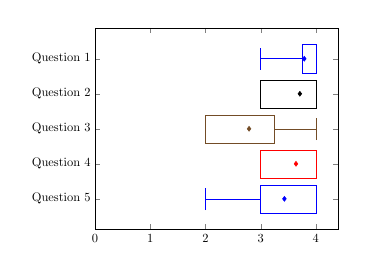
\begin{tikzpicture}[scale=0.45]
  \begin{axis}
    [
    ytick={1,2,3,4,5},
    yticklabels={Question 5, Question 4, Question 3, Question 2, Question 1},
    xmin=0
    ]
    \addplot+[
    boxplot prepared={
      average=3.43,
      upper quartile=4.0,
      lower quartile=3.0,
      upper whisker=4.0,
      lower whisker=2.0
    },
    ] coordinates {};
    \addplot+[
    boxplot prepared={
      average=3.64,
      upper quartile=4.0,
      lower quartile=3.0,
      upper whisker=4.0,
      lower whisker=3.0
    },
    ] coordinates {};
    \addplot+[
    boxplot prepared={
      average=2.79,
      upper quartile=3.25,
      lower quartile=2.0,
      upper whisker=4.0,
      lower whisker=2.0
    },
    ] coordinates {};
    \addplot+[
    boxplot prepared={
      average=3.71,
      upper quartile=4.0,
      lower quartile=3.0,
      upper whisker=4.0,
      lower whisker=3.0
    },
    ] coordinates {};
    \addplot+[
    boxplot prepared={
      average=3.79,
      upper quartile=4,
      lower quartile=3.75,
      upper whisker=4.0,
      lower whisker=3.0
    },
    ] coordinates {};
  \end{axis}
\end{tikzpicture}
\caption{From 14 \system users}
\label{fig:survey1}
\end{subfigure}
~
\begin{subfigure}[t]{0.45\linewidth}
    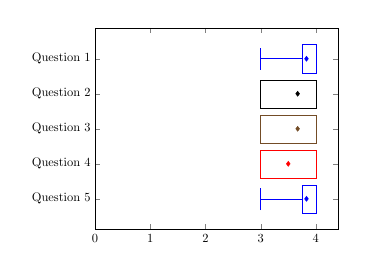
\begin{tikzpicture}[scale=0.45]
  \begin{axis}
    [
    ytick={1,2,3,4,5},
    yticklabels={Question 5, Question 4, Question 3, Question 2, Question 1},
    xmin=0
    ]
    \addplot+[
    boxplot prepared={
      average=3.83,
      upper quartile=4,
      lower quartile=3.75,
      upper whisker=4.0,
      lower whisker=3.0
    },
    ] coordinates {};
    \addplot+[
    boxplot prepared={
      average=3.5,
      upper quartile=4.0,
      lower quartile=3.0,
      upper whisker=4.0,
      lower whisker=3.0
    },
    ] coordinates {};
    \addplot+[
    boxplot prepared={
      average=3.67,
      upper quartile=4.0,
      lower quartile=3.0,
      upper whisker=4.0,
      lower whisker=3.0
    },
    ] coordinates {};
    \addplot+[
    boxplot prepared={
      average=3.67,
      upper quartile=4.0,
      lower quartile=3.0,
      upper whisker=4.0,
      lower whisker=3.0
    },
    ] coordinates {};
    \addplot+[
    boxplot prepared={
      average=3.83,
      upper quartile=4,
      lower quartile=3.75,
      upper whisker=4.0,
      lower whisker=3.0
    },
    ] coordinates {};
  \end{axis}
\end{tikzpicture}
\caption{From 6 \system developers}
\label{fig:survey2}
\end{subfigure}
\caption{Survey results}
 \vspace{-3.0ex} 
\end{figure}

Figure~\ref{fig:survey1} shows the results of the user survey. We can see that most users find \system very useful to locate the root cause. The average score for Question 1 is 3.79, and 11 out of 14 participants find \system very helpful. As for Question 3, \system saves the triage time by 25-50\%. Even in cases that \system cannot correctly locate the root cause, it is still helpful to provide information for further investigation with an average score of 3.43 in Question 5.

For the developer survey, we ask the 6 developers the following 5 questions (Questions 2-5 have the same choices as Question 1):
\begin{itemize}
    \item \textbf{Question 1.} Overall, how convenient is it to change and customize events/rules/domains while using  \system? Answer choices: Convenient(4), Somewhat Convenient(3), Not Convenient(2), Difficult(1).
    \item \textbf{Question 2.} How convenient is it to \emph{change/customize event models} while using \system? 
    \item \textbf{Question 3.} How convenient is it to \emph{add new domains} while using \system? 
    \item \textbf{Question 4.} How convenient is it to \emph{change/customize causality rules} while using \system? 
    \item \textbf{Question 5.} How convenient is it to change/customize \system compared to other SRE tools? 
\end{itemize}

Figure~\ref{fig:survey2} shows the results of the developer survey. Overall, most developers find it convenient to make changes on and customize events/rules/domains in \system. %all questions have very positive responses on average. 5 out of 6 participants find it convenient to make changes on events/rules/domains in \system, while one finds it somewhat convenient. 
% (here domain denotes adding services from different function fields). %We see 3 participants find it somehow convenient in rule customization, indicating that we should make the rule customization easier to use.

\subsection{Lessons learned}
In this section, we share the lessons learned in terms of technology transfer and adoption on using \system in production environments.

\emph{Embedded in Practice.} To build a successful RCA tool in practice, it is important to embed the R\&D efforts in the live environment with SRE experts and users. We have a 30-minute routine meeting daily with an SRE team to manually test and review every site incident. In addition, we actively reach out to the end users for feedback. For example, the users found our initial UI hard to understand. Based on their suggestions, we have introduced alert enrichment with the detailed context of most events, raw metrics, and links to other tools for the next steps. We also make the UI interactive and build user guides, training videos, and sections. As a result, \system has become increasingly practical and well adopted in practice. We believe that R\&D work on observability should be incubated and grown within daily SRE environments. It is also vital to bring developers with rich RCA experience into the R\&D team.

\emph{Vertical Enhancements.} High-confidence and automated vertical enhancements can empower great experiences. \system is enhanced and specialized in critical scenarios such as grouped related %connection stacking 
alerts across services or critical business domain issues, and large-scale scenarios such as infrastructure changes or database issues. Furthermore, the end-to-end automation is also built for integration and efficiency with anomaly detection, RCA, and notification. For notification, domain business anomalies and diagnostic results are sent through communication apps (e.g., slack and email) for better reachability and experience. Within 18 months of R\&D, \system now supports 18 business domains and sub-domains of the company. On average, \system UI supports more than 50 active internal users, and the service sends thousands of results every month. Most of these usages are around the vertical enhancements. 

%\emph{Vertical Enhancement}: During the continued improvements and validations, high accuracy and recurrence scenarios were discovered and enhanced. We created high confidence vertical enhancements that boosted the user's trust and adoption rate. One example here is to use \system for grouped similar connection stacking alerts across the applications or critical domain issues. Thanks to the high customizability of \system, we efficiently enhanced the vertical experiences, such as fine-tuning and specialized events. We then created an end-to-end flow that includes detection, RCA, and notification. Lots of essential incidents with complicated context were supported, such as infra change and database issues. Then, overall efficiency is improved through integrations with other critical site tools. We also attach diagnostic results in the communication apps (e.g., slack, email, and ServiceNow) for better visibility and reachability. Within 18 months of R\&D, we have hundreds of users per month access to the application for 18 domains and sub-domains RCA. We believe for any AIOPs product like \system - vertical enhancements which focus on the domain use cases are essential to success. 


\emph{Data and Tool Reliability.} Reliability is critical to \system itself and requires a lot of attention and effort. For example, if a critical event is missing, \system may infer a totally different root cause, which would mislead users. %the whole causality of an incident may be affected. In this case, it is not helpful that the user can assume only the related metrics/status are fine. 
We estimate the alert accuracy 
%($f1$) 
to be greater than 0.6 in order to be useful. Recall is even more important since \system can effectively eliminate false positive alerts based on the casual ranking. Since there are hundreds of different metrics supported in \system, we spend time to ensure a robust back end by adding partial and dynamic retry logic and high-efficiency cache. \system's unsuccessful cases can be caused by imperfect data, flawed algorithms, or simply code defects. To better trace the reason behind each unsuccessful case, we add a tracing component. Every \system request can be traced back to atomic actions such as retrieving data, data cleaning, and anomaly detection via algorithms.

\emph{Trade-off among Models.} The accuracy and scalability trade-off among anomaly detection models should be carefully considered and tested. In general, some algorithms such as deep-learning-based or ensemble models are more adaptive and accurate than typical ones such as traditional ML or statistical models. However, the former requires more computation resources, operational efforts, and additional system complexities such as training or model fine-tuning. Due to the actual complexities and fast-evolving nature of our context, it is not possible to scale each model (e.g., deep-learning-based models), nor have it deeply customized for every metric at every level. Therefore, while selecting models, we must make careful trade-off in aspects such as accuracy, scalability, efficiency, effort, and robustness. In general, we first set different ``acceptance'' levels by analyzing each event's impact and frequency, and then test different models in staging and pick the one that is good enough. For example, a few alerts such as ``high thread usage'' are defined by thresholds and work just fine even without a model. Some alerts such as  ``service client error'' are more stochastic and require coverage on every metric of every service, and thus we select fast and robust statistical models and actively conduct detection on the fly.  %Business and domain anomaly events can trigger our triaging flow and diagnostics automatically. SRE and monitoring teams spend more time for better and accurate results, such as exercising deep learning approaches, manually correlate critical signals and active improvements for the false positives.

\emph{Phased Incorporation of ML.} In the current industrial settings, ML-powered RCA products still require effective knowledge engineering. Due to the higher complexity and lower ``signal to noise ratio'' of real production incidents, many existing approaches cannot be applied in practice. We believe that the knowledge engineering capabilities can facilitate adoption of technologies such as AIOps. Therefore, \system is designed to be highly customizable and easy to infuse SRE knowledge and to achieve high effectiveness and efficiency. Moreover, a multi-scenario RCA tool requires various and interpretable events from different detection strategies. Auto-ML-based anomaly detection or unsupervised RCA for large service ecosystems is not yet ready in such context.
% resulting in that taking a general ML model is currently not practical in industrial settings.
As for the path of supervised learning, the training data is tricky to label and vulnerable to potential cognitive bias. 
% from SRE engineers
Lastly, the end users often require complete understanding to fully adopt new solutions, because there is no guarantee of correctness. Many recent ML algorithms (e.g., ensemble and deep learning) lack interpretability. Via the knowledge engineering and graph capabilities, \system is able to explain diversity and causality between ML-model-driven and other types of events. Moving forward, we are building a white-box deep learning approach with causal graph algorithms where the causal link weights are parameters and derivable. 
%, while some are manually tuned or detected by rules for certainty and interpretability. For root cause analysis in practice, taking diversified predictive ML anomalies as the major inputs into another ML layer for  root cause analysis, seems too ideal and difficult as mentioned in Section~\ref{sec:intro}. Additionally, there is also a ``chicken-and-egg'' issue for the supervised learning path: collecting training datasets first can be risky and is hard to happen in the SRE domain. Via a graph-based approach, \system is able to explain how diversified and low-level ML events and their connectivity. Also, it effectively and efficiently solve most of the challenge. Lastly, we are more ready for other intelligent solutions with the dataset of 1000+ real production incidents for training, and our AIOPs infrastructure.

%\section{Discussion}

In this section, we discuss some future extension or improvements on the system. 

As we discussed in Section~\ref{sec:anomalyrelated}, there are many related works for anomaly detection. Some approaches are using adaptive concept drifting, which can self-adapt to the target event without manual tuning~\cite{ma2018robust}. One major burden in our event construction is that we need to build different detection strategies/algorithms for different events, while some events are still needed to be manually tuned or detected by rules. Auto-ML is yet to come for anomaly detection, and the interpretability of the result is also a big challenge for end-to-end usability. The filter range for some events also needs manual tuning which requires large amount of domain expertise and is not robust. As of now, we are investing self-adaptive approaches and building time series metrics anomaly detection platform to reduce the event on-boarding cost. 

Also, our approach, which requires a fair amount of ``one-time" effort, utilizes rules to build links between events. A lot of the rules have similar patterns. Despite that our users prefer to have their own control, rules can be inferred from historical patterns. A great extension to this work is the use of machine learning or grammar inference techniques~\cite{wu2019reinam} to automatically or semi-automatically infer the rules.

%At last, since the framework is robust and generic to many use cases, we are planning to release it as open-source system so that we can allow different kinds of users to customize the system based on their own dependencies/events/domains. This also gives us the chance to further speculate \system's performance under different customized scenarios. 


\section{Summary}

We performed a series of galactic disk $N$-body simulations
to investigate the formation and dynamical evolution of spiral arm 
and bar structures in stellar disks which are embedded in live 
dark matter halos.
We adopted a range of initial conditions where the models have similar halo 
rotation curves, but different masses for the disk and bulge components, 
scale lengths, initial $Q$ values, and halo spin parameters.
The results indicate that the bar formation epoch increases exponentially 
as a function of the disk mass fraction with respect to the total mass at the 
reference radius (2.2 times the disk scale length), $f_{\rm d}$.
This relation is a consequence of swing amplification~\citep{1981seng.proc..111T},
which describes the amplification rate of the spiral arm when it transitions from 
leading arm to trailing arm because of the disk's differential rotation.
Swing amplification depends on the properties that characterize the disk, 
Toomre's $Q$, $X$, and $\Gamma$. The growth rate reaches its maximum
for $1<X<2$,  although the position of the peak slightly depends on $Q$ as well as on
$\Gamma$. We computed $X$ for 
$m=2$ ($X_2$), which corresponds to a bar or two-armed spiral, 
for each of our models and found that this value is related to the bar's
formation epoch.

The bar amplitude grows most efficiently when $1<X_2<2$. For models 
with $1<X_2<2$ the bar develops immediately after the start 
of the simulation. As $X_2$ increases beyond $X_2=2$, the growth rate
decreases exponentially. We find that the bar formation epoch increases
exponentially as $X_2$ increases beyond $X_2=2$, in other words
$f_{\rm d}$ decreases. The bar formation epoch exceeds a Hubble time
for $f_{\rm d}\lesssim 0.35$.

Apart from $X$, the growth rate is also influenced by $Q$ where
a larger $Q$ results in a slower growth. This indicates that the bar formation
occurs later for larger values of $Q$. 
Our simulations confirmed this and showed that for the bar ($m=2$) the growth rate
is predicted by swing amplification and becomes visible when it grows beyond a certain amplitude.

Toomre's swing amplification theory further predicts that
the number of spiral arms is related to the mass of the disk, with
massive disks having fewer spiral arms. In addition, larger $\Gamma$
predicts a smaller number of spiral arms.
We confirmed these relations in our simulations. 
The shear rate ($\Gamma$) also affects the pitch angle of spiral
  arms. We further confirmed that our result is consistent with previous
studies.

We found that the disk-to-total mass fraction ($f_{\rm d}$)
and the shear rate ($\Gamma$) are the most important parameters that determine the
morphology of disk galaxies. 
When juxtaposing our models with the Hubble sequence,
the fundamental subdivisions of (barred-)spiral galaxies with 
massive bulges and tightly wound-up spiral arms from S(B)a to S(B)c is 
also be observed as a sequence in our simulations. Where the models 
with either massive bulges or massive disks have more tightly
wound spiral arms. This is because having both a massive disk and bulge results in 
a larger $\Gamma$, i.e., more tightly wound spiral arms. 


Once the
bar is formed it starts to heat the outer parts of the disk.
From this point onwards, 
the self-gravitating spiral arms disappear.
This may be in part caused by the 
lack of gas in our simulations. 
After the bar grows, we no longer discern  
spiral arms in the outer regions of the disk. This could imply
that gas cooling and star formation are required in order to 
maintain spiral structures in barred spiral galaxies for over 
a Hubble time~\citep{1981ApJ...247...77S,1984ApJ...282...61S}.


Our simulations further indicate that non-barred grand-design spirals are
transient structures which immediately evolve into barred
galaxies. Swing amplification teaches us that a massive disk is
required to form two-armed spiral galaxies. This condition, at the
same time, satisfies the short formation time of the bar structure.
Non-barred grand-design spiral galaxies therefore must evolve into barred
galaxies.  We consider that isolated non-barred grand-design spiral galaxies 
are in the process of developing a bar.





\bibliographystyle{IEEEtran}
\bibliography{references}


\end{document}

